\problemname{Sperhling}

%\illustration{0.42}{egg.png}{Easter Egg with Candy.
%Wikimedia Commons, CC BY-SA 3.0.}

On her spare time Caitlin loves to do speed typing. 
Unfortunately Caitlyn was never good at spelling. 
So what often happens is that Catelin makes a mistake spelling a word, 
and has to go back and fix her typo.
One word in particular that Caitlynn has a hard time spelling is the word \texttt{mischievous}.
Catelyn usually spells it \texttt{mischevious} instead. 
In order to fix this typo, Caytlin needs to do 12 key presses.

\begin{center}

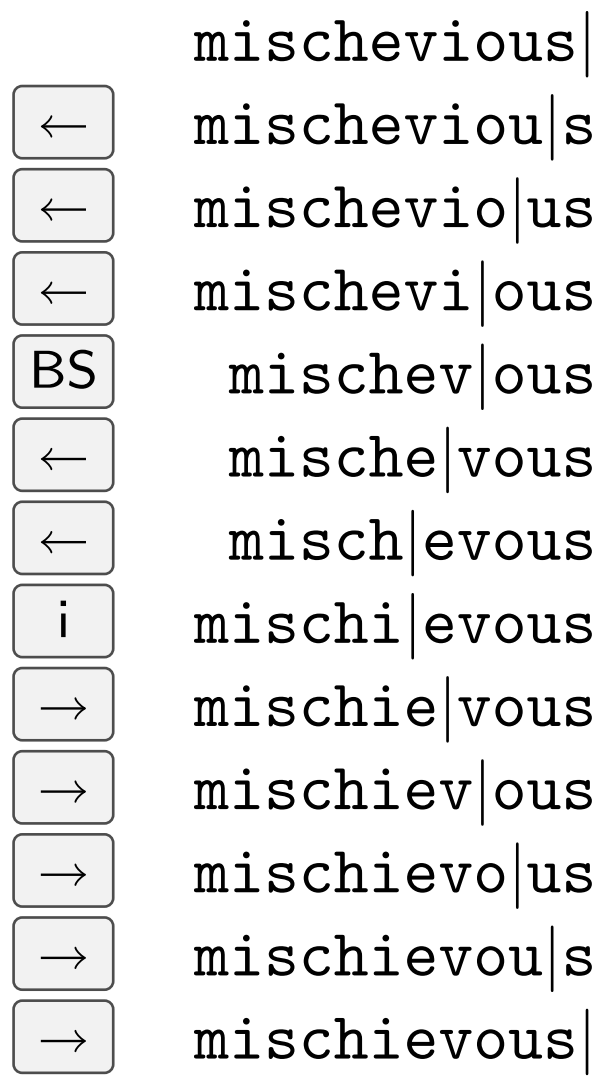
\includegraphics[width=.2\textwidth]{mischievous.png}

\end{center}

%mischevious|
%(left arrow)
%mischeviou|s 
%(left arrow)
%mischevio|us 
%(left arrow)
%mischevi|ous 
%(back space)
%mischev|ous  
%(left arrow)
%mische|vous  
%(left arrow)
%misch|evous  
%(key i)
%mischi|evous 
%(right arrow)
%mischie|vous 
%(right arrow)
%mischiev|ous 
%(right arrow)
%mischievo|us 
%(right arrow)
%mischievou|s 
%(right arrow)
%mischievous| 

Katelin thinks that no matter how much time she puts into speed typing, she will always make mistakes. 
But maybe she can get better at quickly fixing her mistakes. Katelyn would like you to help her with this.

Suppose that Caytlyn has just written the word $S_1$, but that she should have written $S_2$. 
Assume that the cursor is initially at the end of $S_1$, 
and that after fixing the typo, Caitlin needs to place the cursor at the end of $S_2$.
Output the fewest number of key presses needed to make $S_1$ into $S_2$.

The keys you are allowed to use are

\begin{itemize}
	\item the left and right arrow keys.
	\item the back space key.
	\item the keys $\texttt{a}, \ldots, \texttt{z}$.
\end{itemize}

You are not allowed to press back space or the left arrow key when the cursor is all the way to the left. You are also not allowed to press the right arrow key when the cursor is all the way to the right. 

\section*{Input}
The first two lines contain the strings $S_1$ respectively $S_2$. Both $S_1$ and $S_2$ consist only of lowercase English letters, and are between $1$ and $100$ characters long.

\section*{Output}
Output a single line with the fewest number of key presses needed to make $S_1$ into $S_2$.
